\SourcePage{GELFAND-P000470}{unlabelled}
it induces the map $SA\times SA\longrightarrow SA$,
which gives operations on all $K_i$, $i\geqslant0$. (corr. verif. by Whitehead's lemma)
\Unclear{GELFAND-P000470}{whitehead-abbreviation}{The second abbreviation after «корр.» is provisionally read as «прв.».}
\end{GelfandAdjacentEvidence}
\begin{GelfandAdjacentEvidence}{GELFAND-P000470}{2}

They are commutative and agree with those introduced earlier by mutual distributivity, which is verified by Whitehead's lemma.

{\centering\rule{2em}{.4pt}\quad\textperiodcentered\quad\rule{3.4em}{.4pt}\par}
One can define a sum — $H$-space.
On $\widetilde\Omega A$ one can even add an inf. number of matrices!
Hence it will have trivial $K$-functors.
\Unclear{GELFAND-P000470}{omega-mark}{A long wavy mark is written over $\Omega$. It is set as $\widetilde\Omega$.}
\end{GelfandAdjacentEvidence}
\begin{GelfandAdjacentEvidence}{GELFAND-P000470}{3}


{\centering\rule{2.4em}{.4pt}\quad\textperiodcentered\quad\rule{3.1em}{.4pt}\par}
\uuline{\mbox{$K_1A=\pi_0SA$}.}

This is the set of connected components in $GMA$.

$EA$ — the connected component of the identity. (products of \(\underset{\substack{\vert\\\text{\scriptsize pseudotriangular}}}{\text{elem.}}\) matrices),
\SourceFigure{GELFAND-P000470}{pseudo-triangular-insertion}{“Pseudotriangular” is written under “elem.” and connected to it by a stroke.}
\end{GelfandAdjacentEvidence}
\begin{GelfandAdjacentEvidence}{GELFAND-P000470}{4}


\SourceFigure{GELFAND-P000470}{perfectness-hypotheses}{The stepped outline encloses both hypotheses. The arrow starts level with the first one.\par\smallskip\centering
\begingroup\color{black}\GelfandFitDiagram{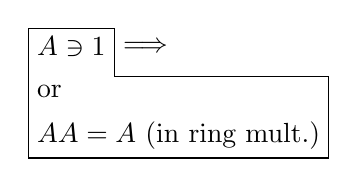
\begin{tikzpicture}[inner sep=3pt]
\node[anchor=west] (unit) at (0,0) {$A\ni1$};
\node[anchor=west] (alt) at (0,-.56) {or};
\node[anchor=west] (idem) at (0,-1.12) {$AA=A$ (in ring mult.)};
\draw (unit.north west) -- (unit.north east) |- (alt.north east -| idem.east)
      -- (idem.south east) -- (idem.south west) -- cycle;
\node[right] at (unit.east) {$\Longrightarrow$};
\end{tikzpicture}}\endgroup}
\end{GelfandAdjacentEvidence}
\begin{GelfandAdjacentEvidence}{GELFAND-P000470}{5}

\[
EA=[GMA,GMA]=[EA,EA].
\]

$K_2A$ — homot. classes of loops. Loops — relations of elem. matrices.

$\Theta A$ has generators $a^{ij}$
\Incomplete{GELFAND-P000470}{middle-generator-cancelled}{The entry after $a^{ij}$ is heavily crossed out. A short leftward arrow is visible below “Loops”.}
\end{GelfandAdjacentEvidence}
\begin{GelfandAdjacentEvidence}{GELFAND-P000470}{6}

(at position $i,j$ stands $a\in A$).

Relations: Steinberg
\[
\begin{gathered}
a^{ij}\ast b^{ij}=(a+b)^{ij},\\
[a^{ij},b^{jk}]=(ab)^{ik}
\end{gathered}
\]
and for some the commutator is $0$.

These are the defining relations.

Let $StA$ — be the group gen. by these generators and relations.
\[
0\longrightarrow K_2A\longrightarrow StA\longrightarrow EA\longrightarrow0
\]
\[
\begin{gathered}
\vert\\[-.2ex]
\text{homot. classes of paths from }0\text{ to somewhere}\\
\text{(with fixed start and end)}
\end{gathered}
\]
\SourceFigure{GELFAND-P000470}{steinberg-paths}{The annotation is connected by a vertical stroke to $StA$.}
\end{GelfandAdjacentEvidence}
\begin{GelfandAdjacentEvidence}{GELFAND-P000470}{7}


{\centering\rule{3.1em}{.4pt}\quad\textperiodcentered\quad\rule{4em}{.4pt}\par}
\Unclear{GELFAND-P000470}{lower-margin-mark}{There is a single retraced mark to the left of the formula. Its reading is unresolved.}
\end{GelfandAdjacentEvidence}
\begin{GelfandAdjacentEvidence}{GELFAND-P000470}{8}

\[
K_2A=\underset{\text{(group homology)}}{\underbrace{H_2EA}}\qquad\sim\qquad
StA=\text{the universal central extension of }EA.
\]

\uline{Problem:} suppose there are 3 matrices in $GMA$. All segments are simplices.
Then all 3 form a simplex.

Generalization: if any pair is a simplex, then all form a simplex.
(space of \uline{tolerance})

{\centering\rule{4em}{.4pt}\quad\textperiodcentered\quad\rule{2.3em}{.4pt}\par}
\uuline{D. A. Kazhdan.}\qquad\uline{Derived category.}

$C$ — an abelian category. Consider the category of complexes $K_C$.
\SourceFigure{GELFAND-P000470}{complexes-diagram}{The arrows point up in both columns. Two arrows point right between the columns.\par\smallskip\centering
\begingroup\color{black}\GelfandFitDiagram{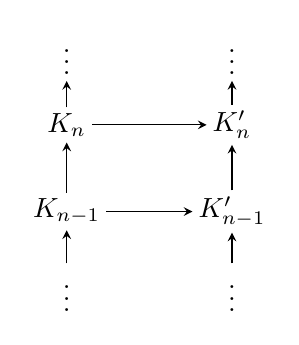
\begin{tikzpicture}[>=stealth,every node/.style={inner sep=2pt}]
\node (l0) at (0,0) {$\vdots$}; \node (r0) at (2.1,0) {$\vdots$};
\node (l1) at (0,-.9) {$K_n$}; \node (r1) at (2.1,-.9) {$K'_n$};
\node (l2) at (0,-2) {$K_{n-1}$}; \node (r2) at (2.1,-2) {$K'_{n-1}$};
\node (l3) at (0,-3) {$\vdots$}; \node (r3) at (2.1,-3) {$\vdots$};
\draw[->] (l1) -- (r1);
\draw[->] (l2) -- (r2);
\draw[->] (l1) -- (l0);
\draw[->] (l2) -- (l1);
\draw[->] (l3) -- (l2);
\draw[->] (r1) -- (r0);
\draw[->] (r2) -- (r1);
\draw[->] (r3) -- (r2);
\end{tikzpicture}}\endgroup}
\end{GelfandAdjacentEvidence}
\begin{GelfandAdjacentEvidence}{GELFAND-P000470}{9}


\Unclear{GELFAND-P000470}{bottom-cancelled-words}{A fragment before “with morphisms” is struck out. A possible reading is «с сост. об.».}
\end{GelfandAdjacentEvidence}
\begin{GelfandAdjacentEvidence}{GELFAND-P000470}{10}

\uline{with morphisms \mbox{$f$} the homot. classes of morphisms of complexes.}
\Unclear{GELFAND-P000470}{bottom-right-cancelled}{A single mark after “morphisms” is struck out. Its reading is unresolved.}
\end{GelfandAdjacentEvidence}
\begin{GelfandAdjacentEvidence}{GELFAND-P000470}{11}

\SourceFigure{GELFAND-P000470}{morphism-underline}{A continuous stepped underline runs beneath the two lines.}
\end{GelfandAdjacentEvidence}
\begin{GelfandAdjacentEvidence}{GELFAND-P000470}{12}


\[
\begin{gathered}
S\subset\operatorname{Hom}K_C\\[-.2ex]
\vert\\[-.2ex]
\text{morph. inducing an isomorphism of homologies}
\end{gathered}
\]
\SourceFigure{GELFAND-P000470}{homology-label}{The annotation is connected by a vertical stroke to $S$.}
\end{GelfandAdjacentEvidence}



\Needspace{7\baselineskip}
\begin{GelfandAdjacentEvidence}{GELFAND-P000471}{1}
